\documentclass{article}
\usepackage[utf8]{inputenc}
\usepackage{graphicx}

\title{WASP: AIML Module 2}
\date{June 2022}

\begin{document}

\maketitle

\section{Logistic Regression}
Logistic regression uses an s-shaped function that maps a set up inputs to a value between 0 and 1, defined by:
$$
p(y = 1| t) =  \frac{e^z}{1 + e^z}
$$
where $z$ is a function, of some weights, inputs and biases ($ w, x, b$, respectively), such that
$$
z(x) = w \cdot x + b
$$
and 
$$
y(x) = 0 \textrm{ if } z(x) < .5, \textrm{ else } 1
$$
The loss can be defined as:
$$
L(x) = \frac{1}{n} \sum_{i = 1}^n log \bigg( 1 + e ^{-y_i(x)} \bigg)
$$
where n is the number of samples. Our objective is to minimize the total loss across all of the samples by changing the parameters $w, b$. Since this function is `nice' in the Calculus sense, we can minimize it analytically, using the gradient.

\subsection{Gradient}

To generalize this further, for any $z(x) = \theta \cdot x$
$$
log(p(x)) = log \bigg( \frac{1}{1+e^{-\theta x}} \bigg)= -log \bigg( 1 + e^{^-\theta x} \bigg)
$$
which yields
$$
L(x) = \frac{1}{n} \sum_{i = 1}^n -log \bigg( y_i \cdot \theta \cdot  x_i -log(1 + e ^-\theta x)  \bigg).
$$
Therefore
$$
\frac{\partial}{\partial \theta_j} y_i \cdot \theta \cdot x_{i,j} = y_i \cdot x_{i,j}
$$
and 
$$
\frac{\partial}{\partial \theta_j} -log(1 + e ^-\theta x)  = x_{j,i}z(x_i)
$$
such that
$$
\frac{\partial}{\partial \theta_j} = L(\theta) \frac{1}{n} \sum_{i = 1}^m(z(x^i) - y^i) \cdot x_{i,j}
$$

\section{Experiments}
I looked at both the feature mapping experiments as well as the learning rate experiments. 

\subsection{Feature Mapping}
In this experiment, we used the original feature map to derive two more based on power transformations of the original data using powers 2 and 3 respectively.

\begin{figure}[h]{
    \centering
    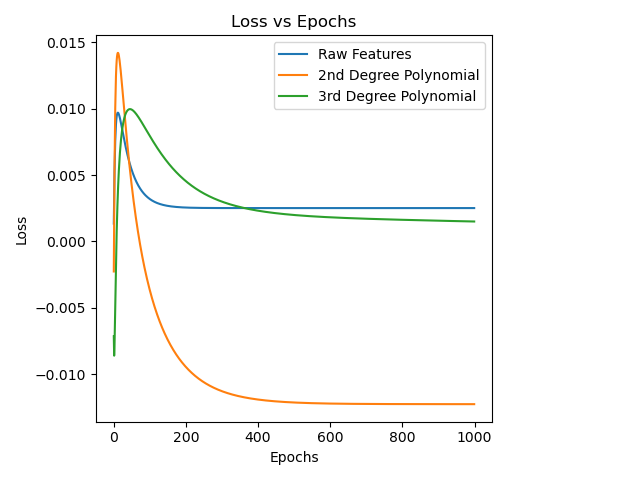
\includegraphics[width=.8\textwidth]{loss_poly.png}
    \caption{Pictured are three logistic regression models that are trained on various power transformations of the data. As we can see}
    \label{fig:my_label}
    }
\end{figure}

\subsection{Learning Rate}

\begin{figure}[h]{
    \centering
    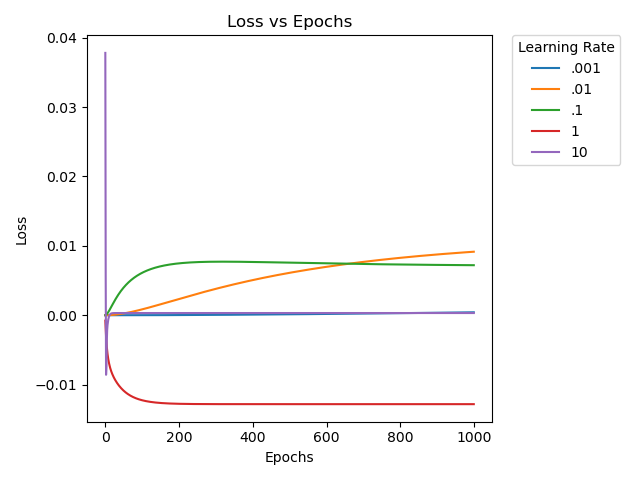
\includegraphics[width=.8\textwidth]{learning_rate.png}
    \caption{Pictured are three logistic regression models that are trained using various learning rate strategies. As we can see, the raw features and the 3rd degree features converge faster, but they all converge on roughly the same loss, which a slight disadvantage to the 2nd degree transformation.}
    \label{fig:my_label}
    }
\end{figure}

\begin{figure}[h]{
    \centering
    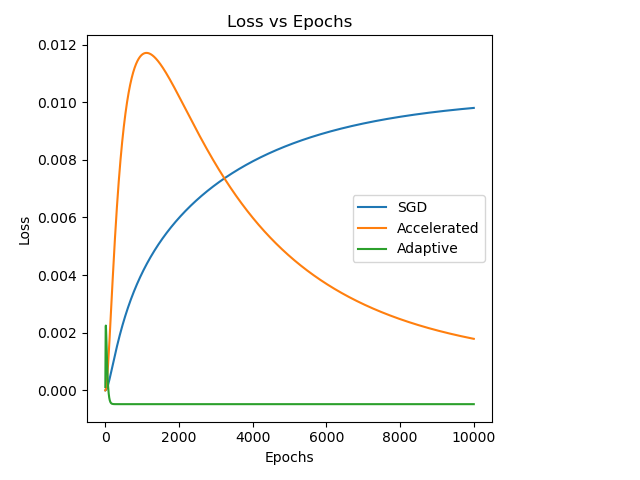
\includegraphics[width=.8\textwidth]{loss.png}
    \caption{Pictured are three logistic regression models that are trained using various learning rate strategies. As we can see, the adaptive method converges incredibly quickly and nearly to zero while the adaptive method lags behind. The stochastic gradient technique performs the worst, due to the fixed step size preventing a smaller loss.}
    \label{fig:my_label}
    }
\end{figure}

\begin{figure}[h]{
    \centering
    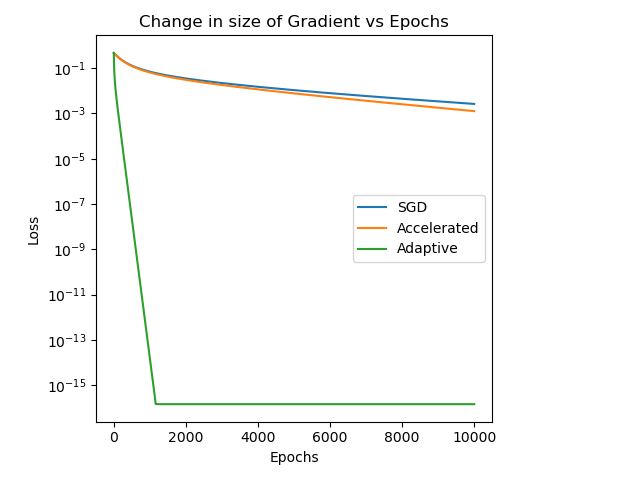
\includegraphics[width=.8\textwidth]{gradient_size.png}
    \caption{Pictured are three logistic regression models that are trained using various learning rate step sizes. The accelerated method takes marginally less time than the stochastic gradient method with a step size = 10 (as optimized above). The adaptive method, however, is much faster.}
    \label{fig:my_label}
    }
\end{figure}





\end{document}
